\documentclass[12pt]{article}

% MLA format
\usepackage[letterpaper]{geometry}
\usepackage{times}
\geometry{top=1.0in, bottom=1.0in, left=1.0in, right=1.0in}
\usepackage{fancyhdr}
\pagestyle{fancy}
\lhead{} 
\chead{} 
\rhead{Simmons \thepage} 
\lfoot{} 
\cfoot{} 
\rfoot{}
\renewcommand{\headrulewidth}{0pt} 
\renewcommand{\footrulewidth}{0pt} 

\usepackage{mdwlist}
\usepackage{enumitem}
\setlist{  
  listparindent=\parindent,
  parsep=0pt,
}
\title{Homework 5A}
\author{Mark Simmons}
\date{March 6, 2020}

% Multi-line glosses
%\usepackage{chngcntr}
%\usepackage{gb4e,cgloss4e}

%\newcounter{glossnum}

%\newcommand{\numgloss}{\refstepcounter{glossnum}\alph{glossnum}.\space}
%\counterwithin{glossnum}{xnumi}
%\renewcommand{\theglossnum}{\thexnumi\alph{glossnum}}

% Typing in IPA
\usepackage{tipa}

% Sentence trees
\usepackage{tikz-qtree}
\usepackage{lscape}
\usepackage{graphicx}
\tikzset{level distance=30pt,
    sibling distance=6pt,
    every tree node/.style={align=center},
    }

\begin{document}

\maketitle

\begin{enumerate}

% question 1
\item Complements and Adjuncts\\
The following sentence has two prepositional phrases within the VP.
\begin{enumerate}
\item John gave the basket of muffins \emph{to Sandy} {\bf{for Mary}.}
\suspend{enumerate}

I claim that the PP \emph{to Sandy} is a complement of the verb \emph{give}, while \emph{for Mary} is an adjunct of the verb.

In sentence (1a), the PP \emph{to Sandy} is obligatory for the verb \emph{give} to form a grammatical sentence, as shown in (1b). (1c) further demonstrates that the preposition \emph{to} is morphologically conditioned and cannot be replaced with any other.
\resume{enumerate}
\item *John gave the basket of muffins for Mary.
\item *John gave the basket of muffins from/at/on Sandy for Mary.
\suspend{enumerate}

The PP \emph{for Mary} in (1a), however, is not obligatory. Sentence (1d) demonstrates that the sentence is fully grammatical with this PP omitted.
\resume{enumerate}
\item John gave the basket of muffins to Sandy.
\suspend{enumerate}

Furthermore, \emph{do-so} replacement allows for the argument \emph{for Mary} to be stranded, but not \emph{to Sandy}.
\resume{enumerate}
\item John gave the basket of muffins to Sandy for Mary, and Jim did so for Susan.
\item *John gave the basket of muffins to Sandy for Mary, and Jim did so to Mary for Susan.
\suspend{enumerate}
Sentence (1h) is similar in structure to (1a).
\resume{enumerate}
\item John blamed his problems \emph{on Mary} \bf{on Tuesday.}
\suspend{enumerate}

I claim that the PP \emph{on Mary} is a complement of the verb \emph{blamed} while the PP \emph{on Tuesday} is an adjunct of the verb.
The PP \emph{on Mary} is required for the sentence to be grammatical, whereas \emph{on Tuesday} can be omitted.
\resume{enumerate}
\item ?John blamed his problems {\bf{on Tuesday}}.
\item John blamed his problems \emph{on Mary}.
\suspend{enumerate}

Sentence (1h) is only acceptable if the PP \emph{on Tuesday} has the same semantic structure as \emph{on Mary} - specifically, that \emph{Tuesday} no longer refers to a temporal theme for the verb, but rather becomes the recipient of the blaming.

Furthermore, the preposition in \emph{on Mary} is conditioned by the verb \emph{blamed} and cannot be substituted by any other, whereas the preposition \emph{on} from \emph{on Tuesday} can be replaced by another and still denote the temporality of the action.
\resume{enumerate}
\item *John blamed his problems at/in/to Mary on Tuesday.
\item John blamed his problems on Mary for three days.
\suspend{enumerate}

% question 2
\item Complements of Adj Heads\\
Part 1.
\begin{itemize}[leftmargin=*]
\item[] \emph{Delightful}\\
The adjective \emph{delightful} can take an optional CP complement, as shown in (2a,b).
\begin{enumerate}
\item This movie is delightful.
\item This movie is delightful \emph{to watch}.
\suspend{enumerate}

I propose that the CP \emph{to watch} is a complement of the Adj \emph{delightful}. Our rules for forming an AdjP predict that CPs can only occur in complement position within the phrase. Furthermore, the CP cannot be stranded in instances of ellipsis.
\resume{enumerate}
\item This movie is delightful to watch, and so is that one.
\item *This movie is delightful to watch, and so is that one \emph{to watch}.
\item *This movie is delightful to watch, and that book \emph{to read}.
\suspend{enumerate}

\item[] \emph{Familiar}\\
The adjective \emph{familiar} can take an optional PP complement, as below.
\resume{enumerate}
\item I'm familiar with math.
\item You have a familiar face.
\suspend{enumerate}

In fact, the adjective has a different semantic sense when used in a copular clause without a complement (but not so in non-copular clauses).
\resume{enumerate}
\item Bob is familiar.
\item Bob looks familiar.
\suspend{enumerate}

In (2h), \emph{familiar} has the meaning of "(inappropriately) familiar or friendly" whereas in (2f,g,i) it has the meaning "acquainted, known." (2j,k) demonstrate further usage of the PP complement introduced by \emph{with}.
\resume{enumerate}
\item Are you familiar with how to write a syntax paper?
\item Steve is familiar with \LaTeX .
\item *Steve is familiar in/about/for \LaTeX .
\suspend{enumerate}

Sentence (2l) demonstrates that the adjective \emph{familiar} conditions the preposition \emph{with} and does not accept any other. This, as well as the semantic distribution of the adjective \emph{familiar}, suggest that it takes a PP complement introduced by \emph{with}.
\item[] \emph{Sensitive}\\
The adjective \emph{sensitive} frequently takes a PP adjunct introduced by \emph{to}.
\resume{enumerate}
\item These old photographs are sensitive to light.
\item \emph{Mimosa pudica} is sensitive to touch.
\suspend{enumerate}
The semantics of the adjective itself are largely the same with or without the adjunct.
\resume{enumerate}
\item Bob is sensitive.
\item Bob is sensitive to criticism.
\suspend{enumerate}

Both adjectives denote that the NP is readily responsive or affected, the adjunct merely specifies what stimulus the NP is affected by. Sentence (r) demonstrates that the PP can be stranded, suggesting its status as adjunct.
\resume{enumerate}
\item I'm sensitive to noise, and my sister is too.
\item I'm sensitive to noise, and my sister to sound.
\suspend{enumerate}
\item[] \emph{Adjacent}
The adjective \emph{adjacent} takes a PP complement introduced by \emph{to}.
\resume{enumerate}
\item The barn is adjacent to the silo.
\suspend{enumerate}
When the adjective occurs without a complement, it is implied that the NP is adjacent to the current space of reference.
\resume{enumerate}
\item The barn's over there. The silo's adjacent (to it).
\suspend{enumerate}

This could be analyzed as ellipsis, in which case the complement would actually be obligatory in copular constructions. In attributive usage, the complement is not necessary.
\resume{enumerate}
\item You can find towels in the adjacent room.
\suspend{enumerate}

Nevertheless, the adjective has the same entailment that the NP it refers to is adjacent to space of reference, here the room in which (2u) was uttered. There are no semantics that allow for a place to be \emph{adjacent} without reference to another place, thus motivating a complement to express this relation.
\item[] \emph{Full}
The adjective \emph{full} takes an optional PP complement introduced by \emph{of}.
\resume{enumerate}
\item The box is full.
\item The box is full of bricks.
\suspend{enumerate}

As stated in Carnie (2007), \emph{of} is the most common preposition to introduce complements. Furthermore, the following sentences demonstrate that it is required to go before any adjuncts.
\resume{enumerate}
\item The box is full to bursting.
\item The box is full of bricks to bursting.
\item *The box is full to bursting of bricks.
\suspend{enumerate}
\end{itemize}
\noindent Part 2.\\
\begin{enumerate}
\item \leavevmode\vadjust{\vspace{-\baselineskip}}\newline
%\begin{landscape}
\noindent\resizebox{\textwidth}{!}{\begin{tikzpicture}
{\small \Tree
[.CP {}
[.C' C\\$\emptyset$
[.TP [.NP D\\The [.N' N\\director {} ]%N'
]%NP
[.T' T\\$\emptyset$ 
	[.VP {} [.V' V\\is
	[.AdjP  {} [.Adj'
	[.AdvP {} [.Adv' Adv\\as {} ] ]
	[.Adj'
		[.Adj' Adj\\aware
		[.PP {} [.P' P\\of
			[.NP D\\the [.N' N\\problems {} ]
			]%NP
		]%P'
		]%PP
		]%Adj'
	[.PP {} [.P' P\\as
		[.NP D\\the [.N'
			[.AdjP {} [.Adj' Adj\\committee {} ]%Adj'
			]%AdjP
			[.N' N\\members {} ]%N'		
		]%N'
		]%NP
	]%P'
	]%PP
	]%Adj'
	]%Adj'
	]%AdjP
	]%V'
	]%VP
]%T'
]%TP
]%C'
]%CP
}
\end{tikzpicture}}

\item \leavevmode\vadjust{\vspace{-\baselineskip}}\newline
%\begin{landscape}
\noindent\resizebox{\textwidth}{!}{\begin{tikzpicture}
{\small \Tree
[.CP {}
[.C' C\\$\emptyset$
[.TP [.NP {} [.N' N\\Everyone {} ]%N'
]%NP
[.T' T\\-ed
	[.VP {} [.V' V\\was
	[.AdjP {}
	[.Adj'
		[.Adj' Adj\\curious
		[.PP {} [.P' P\\about
			[.NP {} [.N' N\\it {} ]
			]%NP
		]%P'
		]%PP
		]%Adj'
	[.PP {} [.P' P\\to
		[.NP D\\the [.N'
			[.AdjP {} [.Adj' Adj\\nth {} ]%Adj'
			]%AdjP
			[.N' N\\degree {} ]%N'		
		]%N'
		]%NP
	]%P'
	]%PP
	]%Adj'
	]%AdjP
	]%V'
	]%VP
]%T'
]%TP
]%C'
]%CP
}
\end{tikzpicture}}
\end{enumerate}

% question 3
\item Argumentation

The most salient feature of phrase heads in X-Bar theory is their required presence for the phrase to be complete and grammatical. However, this presents a dilemma for the analysis of NPs, given that the presumed head, N, is not always required for a full NP, as the data below demonstrate.
\begin{enumerate}[label=(\arabic*)]
\item
\begin{enumerate}[label=\alph*.]
\item I touched those/these/some wires! (overt N)
\item I touched those/these/some! (NP with no overt N)
\end{enumerate}
\suspend{enumerate}

Sentence (1b) suggests that the D argument behaves as a phrase head, given that it occurs both alongside an N, as in (1a), and on its own. However, the reverse scenario is equally possible.
\resume{enumerate}
\item
\begin{enumerate}[label=\alph*.]
\item Those/some cats are cute but lazy.
\item Cats are cute but lazy.
\end{enumerate}
\suspend{enumerate}

As sentence (2b) shows, an N can occur without an accompanying D. Based on obligatoriness alone, therefore, neither D nor N are clearly the phrase head of an NP. However, I will argue based on patterns of morphological inflection, optionality of NP arguments, and distributional equivalence that determiners are overall preferable to nouns as candidate for phrase head of NP.

In X-Bar theory, heads are most likely to be the "morphosyntactic locus" of a phrase. In English, NP elements can be marked for number, definiteness and deixis. The following data show that determiners mark all three features, while nouns only inflect for number.
\resume{enumerate}
\item
\begin{enumerate}[label=\alph*.]
\item I touched the/a wire!
\item I touched the/some wires!
\item That/this dog barked.
\item Those/these dogs barked.
\item That sheep stared at me.
\item Those sheep stared at me.
\end{enumerate}
\suspend{enumerate}

Nouns mark singular and plural morphologically, e.g. \emph{wire/wires} and \emph{dog/dogs}. Several determiners above distinguish number as well, e.g. \emph{this/these} and \emph{that/those}. \emph{a} and \emph{some} are exclusively marked as singular and plural respectively. Only \emph{the} is invariant for either number. Determiners also mark for deixis. \emph{that} and \emph{those} are distal, and \emph{this, these} are proximal. \emph{a} and \emph{some} are both indefinite determiners, while \emph{the} is definite. 

Determiners also inflect for case and gender, though they do so only in the absence of a lexical noun.

\resume{enumerate}
\item
\begin{enumerate}[label=\alph*.]
\item She saw the man.
\item The man saw her.
\item He pet the dog.
\item She pet the dog.
\item The student pet the dog.
\end{enumerate}
\suspend{enumerate}

The determiner \emph{she} in (4a) must be changed to the accusative form \emph{her} in (4b). Notably, the noun \emph{man} in the same sentences does not change form, though it moves from accusative to nominative position. (4c,d) further demonstrate the determiners morphologically express the distinction between male and female referents, while the noun in (4e) is ambiguous with regard to gender.

Thus, determiners bear a significantly heavier morphological load than nouns do by specifying a greater number of features.

Phrase heads also dictate ``optionality and morphology'' of the entire phrase. With regards to the latter, determiners and nouns show agreement with in the number feature.
\resume{enumerate}
\item
\begin{enumerate}[label=\alph*.]
\item That dog barked.
\item Those dogs barked.
\end{enumerate}
\suspend{enumerate}

As discussed above, determiners express a greater breadth of morphological features than nouns, which only mark for number. Thus it is preferable to analyze the determiner as governing the noun morphologically rather than vice versa.

Determiners can also be argued to dictate the optionality of a noun.
\resume{enumerate}
\item
\begin{enumerate}[label=\alph*.]
\item I touched those/these/some wires!
\item I touched those/these/some! (N is optional with these determiners)
\item I touched the/a/no/every wire!
\item *I touched the/a/no/every! (these determiners require an N)
\item He pet the dog.
\item *He man pet the dog. (this determiner forbids an N)
\end{enumerate}
\suspend{enumerate}

The reverse does not appear to be true - apart from personal names, there is no noun that selects only certain determiners.
\resume{enumerate}
\item
\begin{enumerate}[label=\alph*.]
\item The/a certain/every/each person studies syntax.
\item *The/a certain/every/each John studies syntax.
\end{enumerate}
\suspend{enumerate}

For the remainder of this paper we will only discuss non-proper nouns in the interest of not over-complicating our hypothesis.

The rule of government has important implications for the property of distributional equivalence. At first glance, the following sentences seem to suggest that neither determiners nor nouns possess perfect distributional equivalence to a full NP.
\resume{enumerate}
\item
\begin{enumerate}[label=\alph*.]
\item I touched those/these/some!
\item *I touched the/a/no/every!
\item Cats are cute but lazy.
\item *Dog barked.
\end{enumerate}
\suspend{enumerate}

Sentences (8a, c) show that both nouns and determiners can function as a full NP, while (8b, d) show that they cannot always do so. However, if we analyze that determiners govern the optionality of the N argument, then we can explain the ungrammaticality of (8b) - those specific determiners dictate that the N argument is obligatory. Nouns do not have the same lexical selection.

\resume{enumerate}
\item
\begin{enumerate}[label=\alph*.]
\item *Dog/boy slept.
\item The dog/boy slept.
\item Dogs/boys slept.
\item The dogs/boys slept.
\end{enumerate}
\suspend{enumerate}

The ungrammaticality of (9a) does not come from a lexical property of \emph{dog} that prevents from occuring without a determiner. Rather, its conditioned morphologically; (9c) shows that nouns do not need articles when plural and indefinite. Since determiners unambiguously govern nouns at least in morphology, this distributional pattern cannot be an instance of the noun governing the optionality of the determiner, since that would require that the N also govern D morphologically.

This brings us back to the initial dilemma of obligatoriness. We resolved above why some determiners cannot occur without nouns, but why can some plural nouns occur without a determiner? The best analysis might be to posit a null determiner, i.e. $\emptyset_{[+plural +indefinite]}$. Unlike how we handled the non-overt T in TP's, we unfortunately cannot argue that the determiner is in reality an affix that lowers to the N. Given that the plural affix \emph{-s} can co-occur with a variety of determiners, it cannot originate from the D position. There is no argument (that I can propose) to independently motivate the existence of this null determiner, but I argue that analyzing it is preferable given the preponderous evidence I have presented showing that determiners show far more head-like behaviors than nouns do.

In summary, I propose that in order to fit the understanding of phrase heads that X-Bar provides, we must analyze the D argument of the NP as head rather than N. I argue this from morphological evidence - D marks far more morphological features than N does - and demonstrate that the seemingly contradictory distribution of D and N can be explained if D is considered condition N as either optional, required or forbidden, and that the apparent instance of a determiner-less NP can be explained by analyzing a phonologically-null determiner.

Interestingly, this makes the structure of the NP overall closer to that of a TP. If we label the phrase headed by D as DP, and assume the N' that was originally complement to D is actually an NP, then we can see the parallelism between the two phrases.\\

{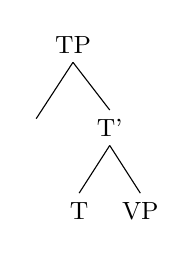
\begin{tikzpicture}
{\small \Tree
[.TP {}
	[.T' T VP ]
]
}
\end{tikzpicture}}
{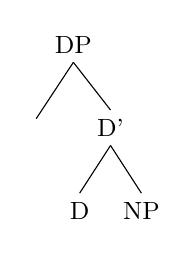
\begin{tikzpicture}
{\small \Tree
[.DP {}
	[.D' D NP ]
]
}
\end{tikzpicture}}

Thus, my argument also provides analytic elegance in unifying disparate phrasal structures.

\item The title is a sentence in French. It idiomatically translates to "What's that?" A morpheme-by-morpheme translation would be "What is that that that is?" This is appropriate given that "that" (\emph{ce}) itself is a determiner, it's like the title is questioning what a determiner is, which is funny because I just spent the past 3 hours writing about what a determiner is.

\end{enumerate}
\end{document}
